% =====================================================================
%  Landscaping Proposal: Manjushree Park & Chobhar Community Forest
%  Worldlink Communications - Environment Day 2026
%
%  Compile with:  pdflatex landscaping.tex   (run twice)
%  Font: Times New Roman (via mathptmx + newtxtext)
% =====================================================================
\documentclass[11pt,a4paper]{article}

% ----- Fonts: Times New Roman -----
\usepackage[T1]{fontenc}
\usepackage[utf8]{inputenc}
\usepackage{mathptmx}      % Times for text + math (Times New Roman family)
\usepackage{amsmath}
\renewcommand{\familydefault}{\rmdefault}

% ----- Geometry & layout -----
\usepackage[a4paper,margin=2.4cm]{geometry}
\usepackage{setspace}
\onehalfspacing
\usepackage{microtype}
\usepackage{parskip}

% ----- Graphics, tables, colors -----
\usepackage{graphicx}
\graphicspath{{Figuress/}{figures/}}

\usepackage{booktabs}
\usepackage{array}
\usepackage{tabularx}
\usepackage{longtable}
\usepackage{multirow}
\usepackage{ragged2e}
\newcolumntype{L}[1]{>{\RaggedRight\arraybackslash}p{#1}}

% ----- Captions & figures -----
\usepackage{float}
\usepackage[font=small,labelfont=bf,labelsep=period]{caption}
\usepackage{subcaption}

% ----- Lists -----
\usepackage{enumitem}
\setlist{itemsep=2pt,topsep=4pt,parsep=0pt}

% ----- Headers / footers -----
\usepackage{fancyhdr}
\pagestyle{fancy}
\fancyhf{}
\fancyhead[L]{\small Manjushree Park Landscaping Proposal}
\fancyhead[R]{\small Worldlink Environment Day 2026}
\fancyfoot[C]{\thepage}
\renewcommand{\headrulewidth}{0.4pt}

% ----- Section style (all black) -----
\usepackage{titlesec}
\titleformat{\section}{\Large\bfseries}{\thesection}{0.6em}{}
\titleformat{\subsection}{\large\bfseries}{\thesubsection}{0.6em}{}
\titleformat{\subsubsection}{\normalsize\bfseries}{\thesubsubsection}{0.6em}{}

% ----- Plain inline note (no colour, no box) -----
% Usage: \begin{notebox}[Title]  text  \end{notebox}
\newenvironment{notebox}[1][Note]{%
  \par\medskip\noindent\textbf{#1.~}\ignorespaces}{\par\medskip}

% ----- Hyperlinks (black) -----
\usepackage[hidelinks]{hyperref}

% =====================================================================
\begin{document}

% -------------------- TITLE PAGE --------------------
\begin{titlepage}
\centering
\vspace*{0.2cm}

\includegraphics[width=0.32\linewidth]{703715117_1103542609513440_9114886208172518010_n.jpg}\\[0.25cm]

{\scshape\large Worldlink Communications Pvt.\ Ltd.\par}
\vspace{0.1cm}
{\scshape Environment Day 2026 \,\textbar\, Corporate Social Responsibility Initiative\par}

\vspace{0.5cm}
\rule{\linewidth}{1.2pt}\\[0.35cm]
{\huge\bfseries Landscaping Proposal\par}
\vspace{0.3cm}
{\Large\itshape Manjushree Park \& Chobhar Community Forest\par}
\vspace{0.15cm}
{\large Three-Site Plantation Plan, Environment Day 2026\par}
\rule{\linewidth}{1.2pt}\\[0.6cm]

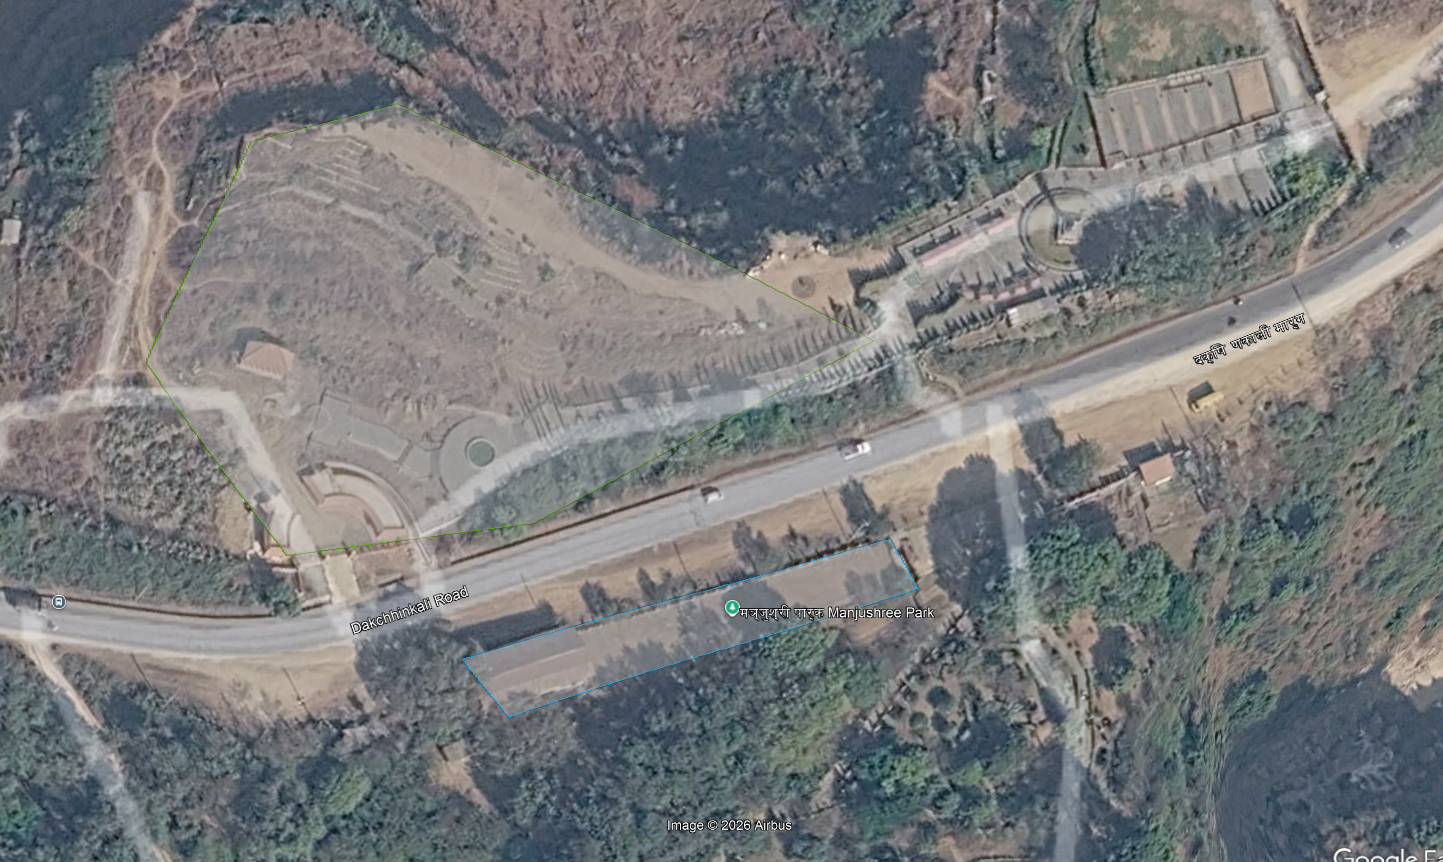
\includegraphics[width=0.45\linewidth]{satellite_manjushree.png}\\[0.25cm]
{\footnotesize\itshape Satellite context of the project area at Chobhar Gorge, Kirtipur. The polygonal outline (upper) traces the community forest cleared zone proposed for Site~2; the rectangular outline (lower, along Dakchhinkali Road) marks the Manjushree Park strip housing the proposed Site~1 Children's Park. Site~3 follows the road frontage between the two outlines.}\\[0.6cm]

\begin{tabular}{rl}
\textbf{Prepared for} & Worldlink Communications Pvt.\ Ltd. \\[2pt]
\textbf{In coordination with} & Manjushree Community Forest User Group (CFUG) \\[2pt]
\textbf{Location} & Chobhar Gorge, Kirtipur Municipality, Bagmati Province, Nepal \\[2pt]
\textbf{Coordinates} & $27.66^{\circ}$\,N, \ $85.29^{\circ}$\,E \ (approx.\ 1{,}350~m a.s.l.) \\[2pt]
\textbf{Approval} & Confirmed by the CFUG President, Manjushree CFUG \\[2pt]
\textbf{Initiative} & Environment Day Plantation 2026 \\
\end{tabular}

\vfill
\rule{\linewidth}{0.6pt}\\[0.25cm]
{\small\scshape Official Project Document \,\textbar\, For Internal \& CFUG Review}
\end{titlepage}

\tableofcontents
\newpage

% =====================================================================
\section{Background}
\label{sec:background}

This document presents a comprehensive landscaping proposal for a plot of land within \textbf{Manjushree Park}, Chobhar, Kirtipur Municipality, Kathmandu Valley. The proposal has been prepared in conjunction with \textbf{Worldlink Communications'} Environment Day plantation initiative, aimed at:
\begin{itemize}
  \item Enhancing green cover and ecological sustainability.
  \item Beautifying the public recreational space through strategic fruit-tree and ornamental selection.
  \item Creating an interactive, edible landscape for park visitors and local wildlife.
\end{itemize}

Manjushree Park holds significant cultural and ecological importance. Established to restore the landscape scarred by a now-defunct cement factory at Chobhar Gorge, the park today serves as a peaceful recreational retreat for both residents and tourists. It is named after \emph{Manjushree}, the Buddhist bodhisattva credited in legend with draining the ancient Nagdaha lake to create the Kathmandu Valley by cutting the Chobhar Gorge.

% =====================================================================
\section{Study Area Description}
\label{sec:study-area}

\subsection{Location \& General Setting}
\begin{description}[leftmargin=3.2cm,style=nextline,font=\normalfont\bfseries]
  \item[Location] Chobhar Gorge, Kirtipur Municipality, Bagmati Province, Nepal.
  \item[Road Frontage] Dakchhinkali Road, a major highway running NW to SE through Chobhar.
  \item[Coordinates] Approximately $27.66^{\circ}$\,N, $85.29^{\circ}$\,E.
  \item[Altitude] Approximately 1{,}350~m above sea level (mid-hill zone).
\end{description}

\begin{figure}[!htbp]
  \centering
  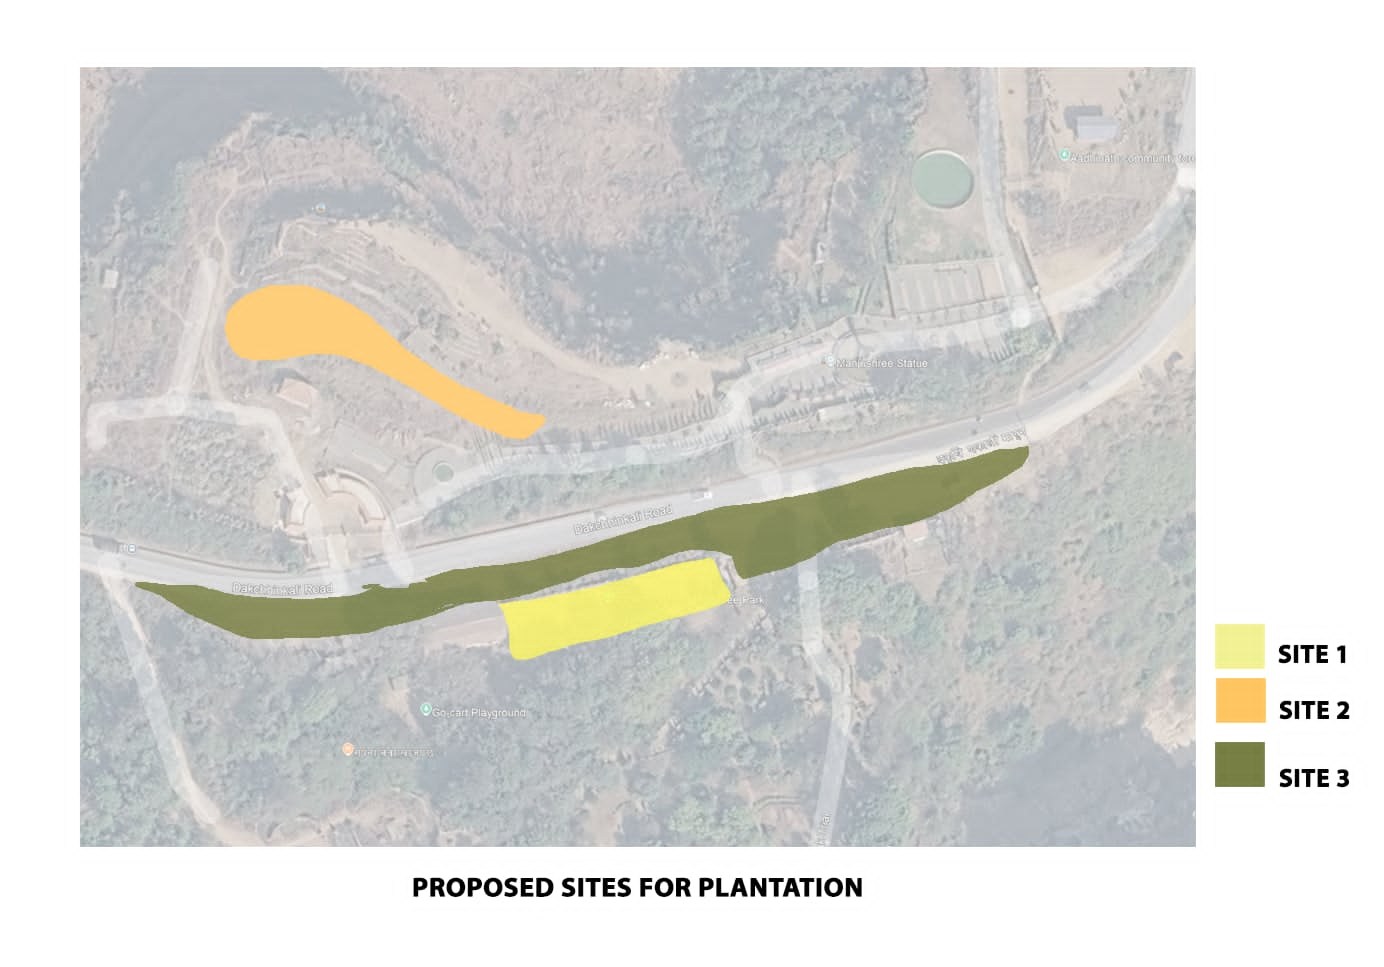
\includegraphics[width=0.82\linewidth]{proposed_sites_overview.jpg}
  \caption{Proposed plantation sites at Chobhar, overlaid on satellite imagery (legend at right of figure). \textbf{Site~1} (yellow) is the small rectangular plot south of Dakchhinkali Road, marked at ``Manjushree Park'', earmarked for the Children's Park. \textbf{Site~2} (orange, kidney-shaped) is the cleared zone north of the road within the community forest, designated for the edge fruit/flowering plantation. \textbf{Site~3} (olive/dark green, long curving strip) follows the Dakchhinkali Road frontage and is the candidate for low shrub planting only, owing to the planned 23~m road widening.}
  \label{fig:sites-overview}
\end{figure}

\subsection{Key Physical Features}
Observations drawn from satellite imagery and field reconnaissance, mapped to the three sites in Figure~\ref{fig:sites-overview}:
\begin{itemize}
  \item \textbf{Dakchhinkali Road} runs NW--SE through the site, separating Site~2 (north of the road, inside the community forest) from Site~1 (south of the road, inside Manjushree Park). It is a two-lane highway planned for widening to a \textbf{23\,m corridor}, which directly drives the Site~3 design.
  \item \textbf{Site~1} (Children's Park): a roughly rectangular cleared plot within Manjushree Park, measuring approximately \textbf{64.6\,m (E--W) $\times$ 10.6--12.6\,m (N--S)}, with a flagstone-paved entrance / gate at the east end.
  \item \textbf{Site~2} (Community Forest): a cleared kidney-shaped zone within the surrounding forest, bordered on all sides by mature canopy that will act as a permanent windbreak and ecological buffer.
  \item \textbf{Site~3} (Roadside): the narrow linear strip immediately along Dakchhinkali Road, sitting within the future 23\,m right-of-way. Overhead power and utility lines follow this corridor, constraining mature height.
  \item Gently sloping terrain (approx.\ 5--8\% gradient) descends from the road toward the forested gorge below; no terracing is required.
  \item A roundabout and park entrance feature is visible at the north-western end of the site, and the dense gorge forest provides a natural backdrop.
  \item The scenic backdrop of Chandragiri and Champadevi hills frames the site to the south-west.
\end{itemize}

\subsection{Climate \& Soil Context}
Kathmandu Valley falls within a \textbf{humid subtropical to warm temperate} climate zone. The area receives approximately \textbf{1{,}400~mm} of rainfall annually, concentrated between June and September (monsoon). Winters are mild with occasional frost at this altitude.

Soils in the Chobhar area are typically \textbf{sandy loam to clay loam}, moderate in organic matter, and slightly acidic to neutral (pH 5.5--7.0), well suited for a wide range of fruit and ornamental trees. A distinctive feature of the Chobhar locality is the presence of \textbf{limestone} in the underlying geology and soil profile, a legacy of the limestone deposits that once supplied the former Himal Cement factory at Chobhar Gorge. As a result, the soil is locally \textbf{calcareous (lime-rich)} and tends slightly toward the alkaline end of the pH range in some pockets. This favours lime-tolerant species such as Guava, Pomegranate, Lapsi and Citrus, which have been prioritised in the species selection for Sites~1 and~2. Soil may also have been historically affected by the cement bunker; visual inspection suggests these effects are not currently significant, but a basic \textbf{pH, free-lime and texture test} prior to planting is recommended.

% =====================================================================
\section{Methodology \& Plant Selection}
\label{sec:methodology}

\subsection{Site Assessment Approach}
The following engineering and horticultural criteria were applied to evaluate species suitability:
\begin{itemize}
  \item Altitude suitability (mid-hill: 1{,}000--2{,}000~m).
  \item Root system type (deep vs.\ shallow, critical near structures and paved areas).
  \item Canopy spread vs.\ available spacing.
  \item Risk classification (road hazard, utility-line interference).
  \item Water requirement and drought tolerance.
  \item Ecological benefit: soil binding, pollinator support, bird habitat.
  \item Community benefit: edible fruit, shade, aesthetics.
\end{itemize}

\subsection{Revised Three-Site Zoning Framework}
Based on field reassessment, the original three-zone framework (A, B, C) within a single strip was found to be \textbf{infeasible}: the strip is too narrow to support distinct front, mid, and rear belts. The proposal has therefore been restructured into a \textbf{three-site plan}, each with a distinct function and design priority (see Figure~\ref{fig:sites-overview}).

\begin{table}[H]
\centering
\small
\begin{tabularx}{\linewidth}{L{2.0cm} L{4.4cm} X}
\toprule
\textbf{Site} & \textbf{Location} & \textbf{Function} \\
\midrule
\textbf{Site~1} & Cleared zone within Manjushree Park, earmarked for a Children's Park ($\sim$64.6\,m $\times$ 11\,m) & \textbf{Natural Playground} centred on log play, sand pits and curvilinear pathways, framed by slender evergreens on the north and a flowering/fruit sensory edge on the south. \\
\textbf{Site~2} & Adjacent Community Forest, cleared zone north of Dakchhinkali Road & Edge plantation of fruit/flowering trees with low hedges for site demarcation and ecological buffer. \\
\textbf{Site~3} & Roadside strip directly along Dakchhinkali Road (future 23\,m road expansion corridor) & Low shrub plantation only, or no plantation, to preserve sightlines and accommodate the future widened road. \\
\bottomrule
\end{tabularx}
\caption{Three-site framework. All three sites have been confirmed by the CFUG President for Environment Day planting.}
\end{table}

\begin{notebox}[Design priority]
Where any earlier zoning concept conflicts with the detailed Children's Park (Site~1) design described in Section~\ref{sec:site1}, the Children's Park design takes precedence. Sites~2 and~3 are supporting plantations around that core.
\end{notebox}

% =====================================================================
\section{Site~1: Children's Park --- Natural Playground}
\label{sec:site1}

\subsection{Design Intent}
Site~1 is the project's centrepiece: a cleared rectangular zone within Manjushree Park (approximately \textbf{64.6\,m long $\times$ 10.6--12.6\,m wide}) developed as a \textbf{Natural Playground for children}. The design deliberately avoids synthetic play structures and plastic toys in favour of timber, sand, stone and living plants. All internal geometry is curvilinear; rigid straight lines are excluded.

\begin{figure}[H]
  \centering
  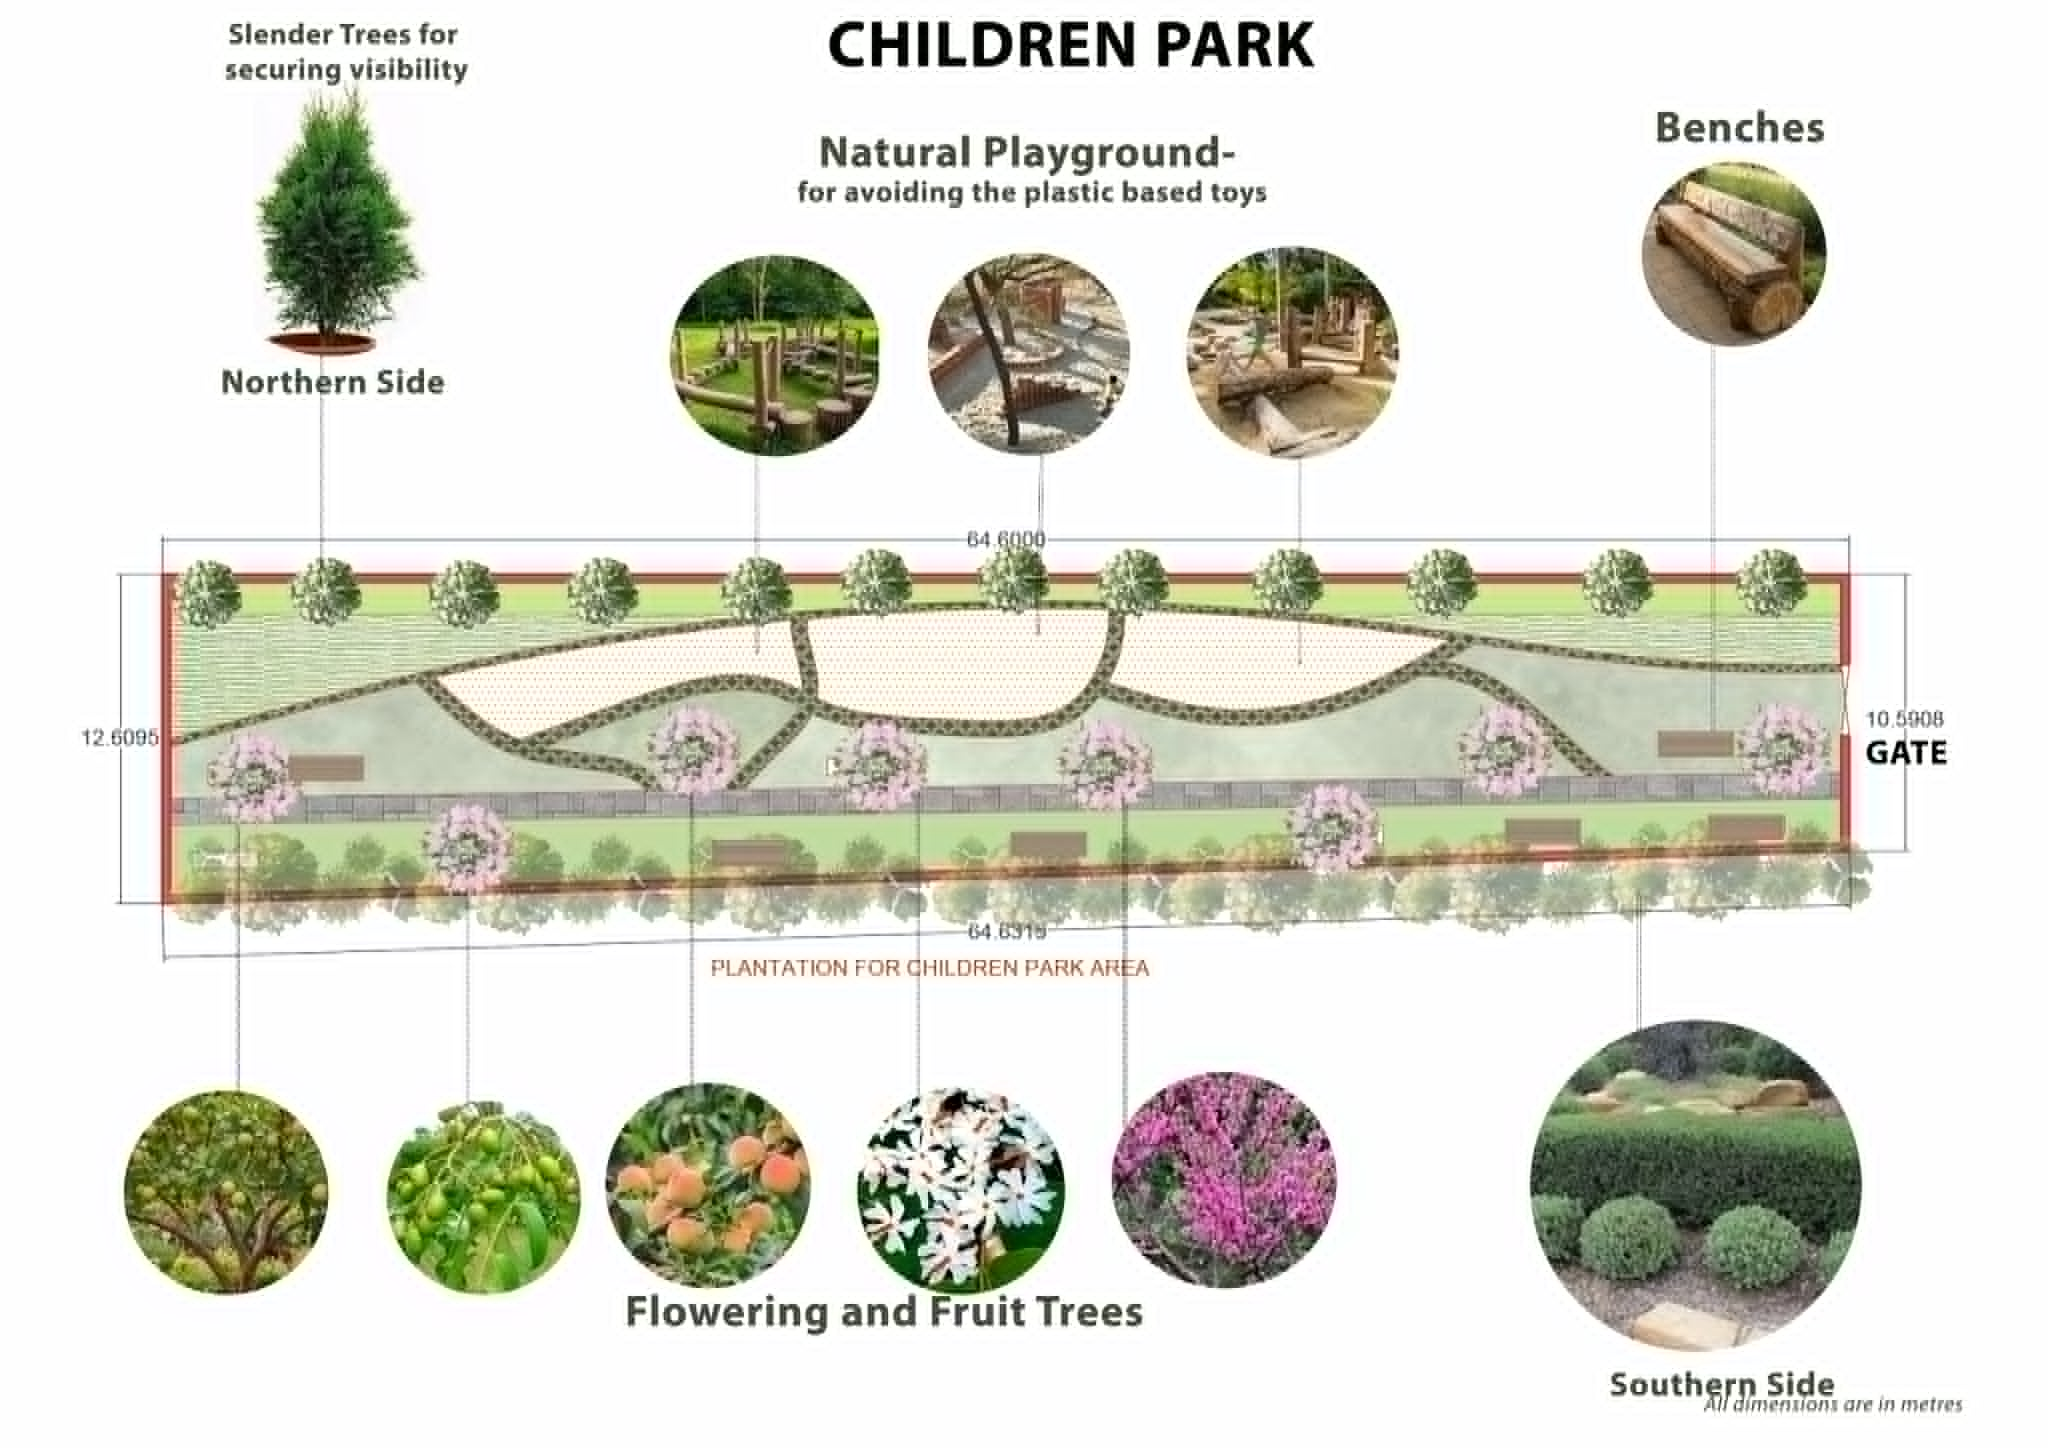
\includegraphics[width=\linewidth]{children_park_plan.jpg}
  \caption{Detailed plan for the Site~1 Children's Park. The plot measures \textbf{64.60~m (E--W) $\times$ 10.59--12.61~m (N--S)}; all dimensions on the figure are in metres. The main \emph{Gate} sits at the east end. The \textbf{northern edge} is lined with slender conical evergreens (``slender trees for securing visibility'') interleaved with low spherical shrubs. The central \textbf{Natural Playground} (annotated with inset photographs of log balancing trails, sand pits and timber climbing frames) occupies curvilinear turf islands separated by organic-shaped sand/gravel zones and a paved walkway. The \textbf{southern edge} is a sensory band of flowering and fruit trees (guava, peach, plus pink and white seasonal bloomers) with a low manicured hedge line at ground level. Rustic log \textbf{benches} are positioned along the walkway and near the gate.}
  \label{fig:children-park}
\end{figure}

\subsection{The Play Zone: Natural Playground}
Positioned centrally within the park, the play area uses natural materials to stimulate physical agility, balance and imaginative play without relying on synthetic structures.
\begin{description}[font=\normalfont\bfseries,leftmargin=2.4cm]
  \item[Log Balancing Trails] Stepping stumps and fallen-log balance beams set over natural turf.
  \item[Sand Play Pits] Organic-shaped sand zones bounded by timber edging for safe, tactile exploration.
  \item[Timber Climbing Frames] Low-impact wooden structures that blend seamlessly into the landscape.
\end{description}

\subsection{Northern Boundary: Slender Tree Demarcation}
The northern edge is lined with a uniform row of \textbf{slender, conical evergreen trees} (e.g.\ \emph{Thuja} or \emph{Cypress}). This row serves a dual purpose: it provides structural framing and a green privacy screen for the park perimeter, while its high canopy and narrow profile preserve clear sightlines so parents can supervise the entire play zone from any point inside the park.

\subsection{Southern Boundary: Sensory \& Fruit Plantation}
The southern edge is a diverse, vibrant buffer designed to offer children a rich sensory and interactive experience.
\begin{itemize}
  \item \textbf{Flowering and fruit trees:} a curated mix of seasonal flowering trees (bright pink and white blooms) together with low-hanging fruit trees such as guava, mango and peach. The result is a shifting palette of colour, fragrance and an educational farm-to-table experience for visiting children.
  \item \textbf{Low hedges:} beneath the canopy, neatly manicured low shrubs and spherical hedges define the southern baseline, adding layers, texture and soft natural containment.
\end{itemize}

\subsection{Circulation \& Amenities}
\begin{description}[font=\normalfont\bfseries,leftmargin=2.8cm]
  \item[Pedestrian Walkway] A linear, paved pathway runs parallel to the southern plantation zone, connecting the main entrance gate to the entire length of the park for easy stroller and wheelchair accessibility.
  \item[Rustic Seating] Heavy-timber log benches are placed along the pathway and under the shade of the flowering trees, offering comfortable resting spots for parents and guardians with direct sightlines onto the central play areas.
\end{description}

\subsection{Geometry \& Layout: Curvilinear Play Areas}
The internal zones, sand pits and pathways are deliberately designed with \textbf{organic, flowing, curvy geometries} rather than rigid straight lines.
\begin{itemize}
  \item \textbf{Encouraging natural movement:} curving paths and edges mimic nature and encourage children to run, explore and play at a relaxed, intuitive pace.
  \item \textbf{Safety and softness:} eliminating sharp corners reduces collision hazards and makes the layout inherently safer for high-energy play.
  \item \textbf{Visual harmony:} the fluid shapes soften the long, narrow constraints of the site, making the park feel wider, more expansive and visually connected to the ``Natural Playground'' theme.
\end{itemize}

\subsection{Recommended Species (Site~1 Edges)}
\begin{table}[H]
\centering
\small
\begin{tabularx}{\linewidth}{L{2.4cm} L{3.0cm} L{3.6cm} X}
\toprule
\textbf{Edge} & \textbf{Role} & \textbf{Indicative Species} & \textbf{Notes} \\
\midrule
Northern & Slender screen / visibility frame & \emph{Thuja occidentalis}, \emph{Cupressus sempervirens} & Uniform conical form, evergreen, 2--3\,m spacing. \\
Southern (canopy) & Sensory \& fruit & Guava (\emph{Amba}), Peach (\emph{Aaru}), Mango (\emph{Aanp}), seasonal flowering ornamentals & Low-hanging fruit safe for children; pink/white blooms. \\
Southern (ground) & Low hedge & \emph{Buxus} spp., \emph{Duranta} dwarf, \emph{Murraya} & Spherical/clipped, 0.4--0.8\,m height. \\
\bottomrule
\end{tabularx}
\caption{Edge planting palette for the Children's Park (Site~1).}
\end{table}

% =====================================================================
\section{Site~2: Community Forest --- Edge Plantation}
\label{sec:site2}

\subsection{Concept}
Site~2 is a cleared zone within the adjacent community forest, north of Dakchhinkali Road. It is developed as an \textbf{edge plantation} to protect future site functions while adding ecological value. Planting fruit or flowering trees along the perimeter creates an engaging sensory experience, while small hedges provide clear, natural demarcation between the cleared zone and the surrounding forest.

\begin{figure}[htbp]
  \centering
  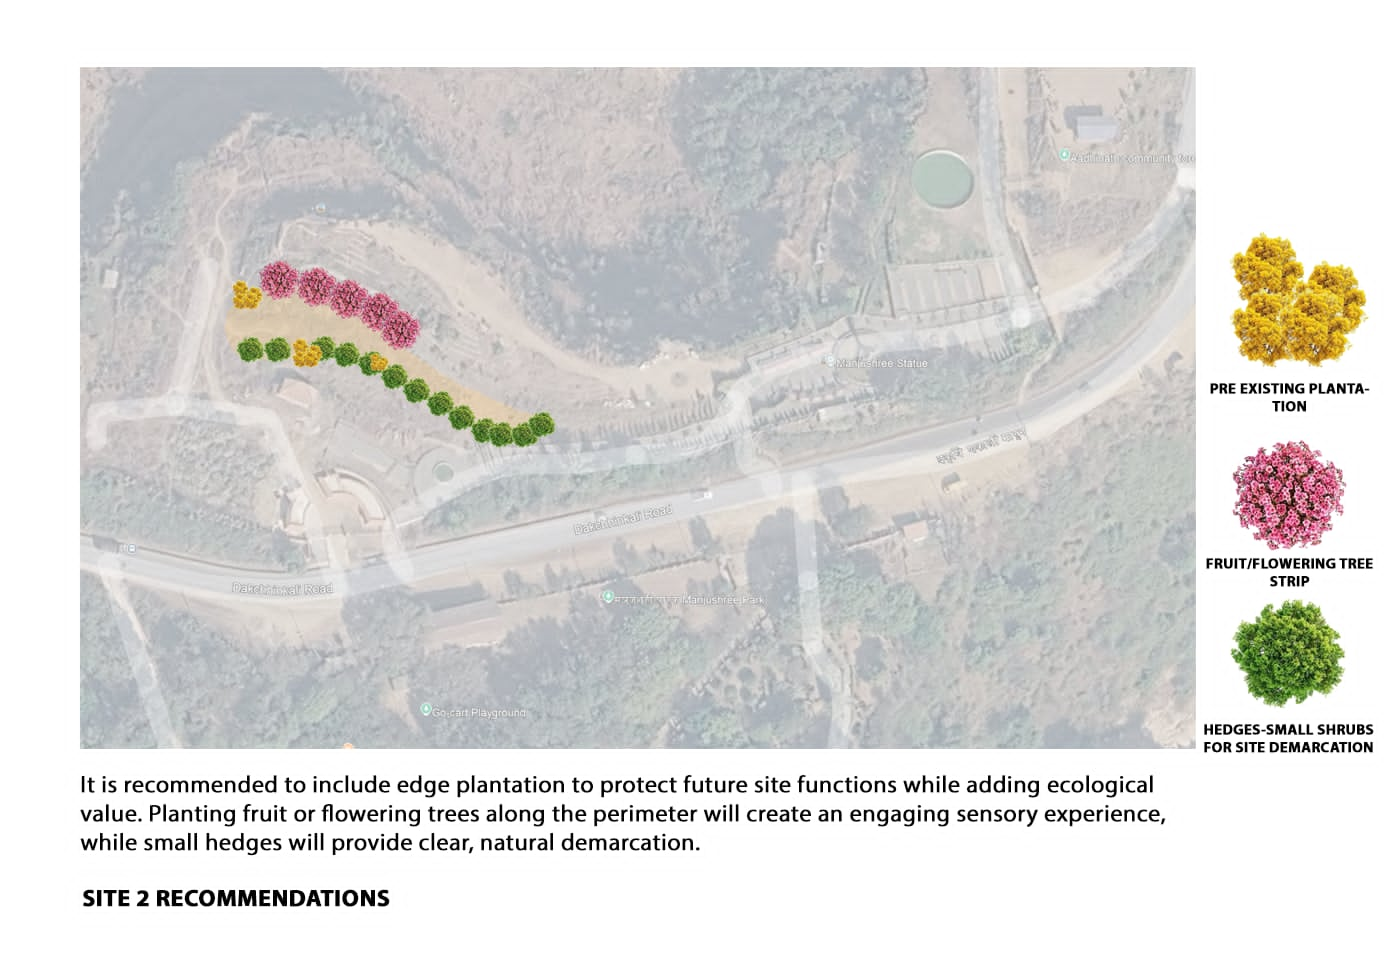
\includegraphics[width=0.78\linewidth]{site2_community_forest.jpg}
  \caption{Site~2 edge plantation recommendation, shown as a three-band layering against the cleared zone in the community forest. The legend (right of figure) identifies: \textbf{yellow} = \emph{pre-existing plantation} (the existing forest canopy, retained as-is), \textbf{pink} = \emph{fruit / flowering tree strip} (the new mid-row to create an engaging sensory perimeter), and \textbf{green} = \emph{hedges and small shrubs for site demarcation} (the outermost line, providing a clear natural boundary between the cleared interior and the forest beyond).}
  \label{fig:site2}
\end{figure}

\subsection{Recommended Species (Site~2)}
\begin{table}[H]
\centering
\small
\begin{tabularx}{\linewidth}{L{2.7cm} L{3.6cm} L{2.2cm} L{1.6cm} X}
\toprule
\textbf{Common} & \textbf{Scientific Name} & \textbf{Local Name} & \textbf{Spacing} & \textbf{Notes} \\
\midrule
Lapsi (Hog Plum) & \emph{Choerospondias axillaris} & Lapsi & 5~m & Indigenous, culturally significant. \\
Pear & \emph{Pyrus communis} & Naspati & 5--6~m & Reliable fruiting in mid-hills. \\
Peach & \emph{Prunus persica} & Aaru & 5~m & Fruits within 2--3 years. \\
Plum & \emph{Prunus salicina} & Aalubakhada & 5~m & Hardy, attractive flowering. \\
Lychee & \emph{Litchi chinensis} & Litchi & 6~m & Thrives in Kathmandu Valley. \\
Guava & \emph{Psidium guajava} & Amba & 5~m & Soil-binding roots, quick fruiting. \\
\bottomrule
\end{tabularx}
\caption{Site~2 fruit / flowering edge species.}
\end{table}

\paragraph{Existing Forest Buffer.} The surrounding community forest is preserved \textbf{as-is}. No clearing is permitted beyond the agreed Site~2 boundary. The dense surrounding canopy acts as a windbreak, maintains soil stability on the gorge slopes and provides natural ecological connectivity.

% =====================================================================
\section{Site~3: Roadside Strip --- Dakchhinkali Road}
\label{sec:site3}

\subsection{Constraints \& Strategy}
Site~3 is the narrow strip directly adjacent to Dakchhinkali Road. The road is planned for a future expansion to a \textbf{23\,m width}, which will typically accommodate higher-speed and higher-volume traffic. Plantation immediately at the road edge may therefore be lost during expansion and could compromise driver visibility in the interim.

\begin{figure}[htbp]
  \centering
  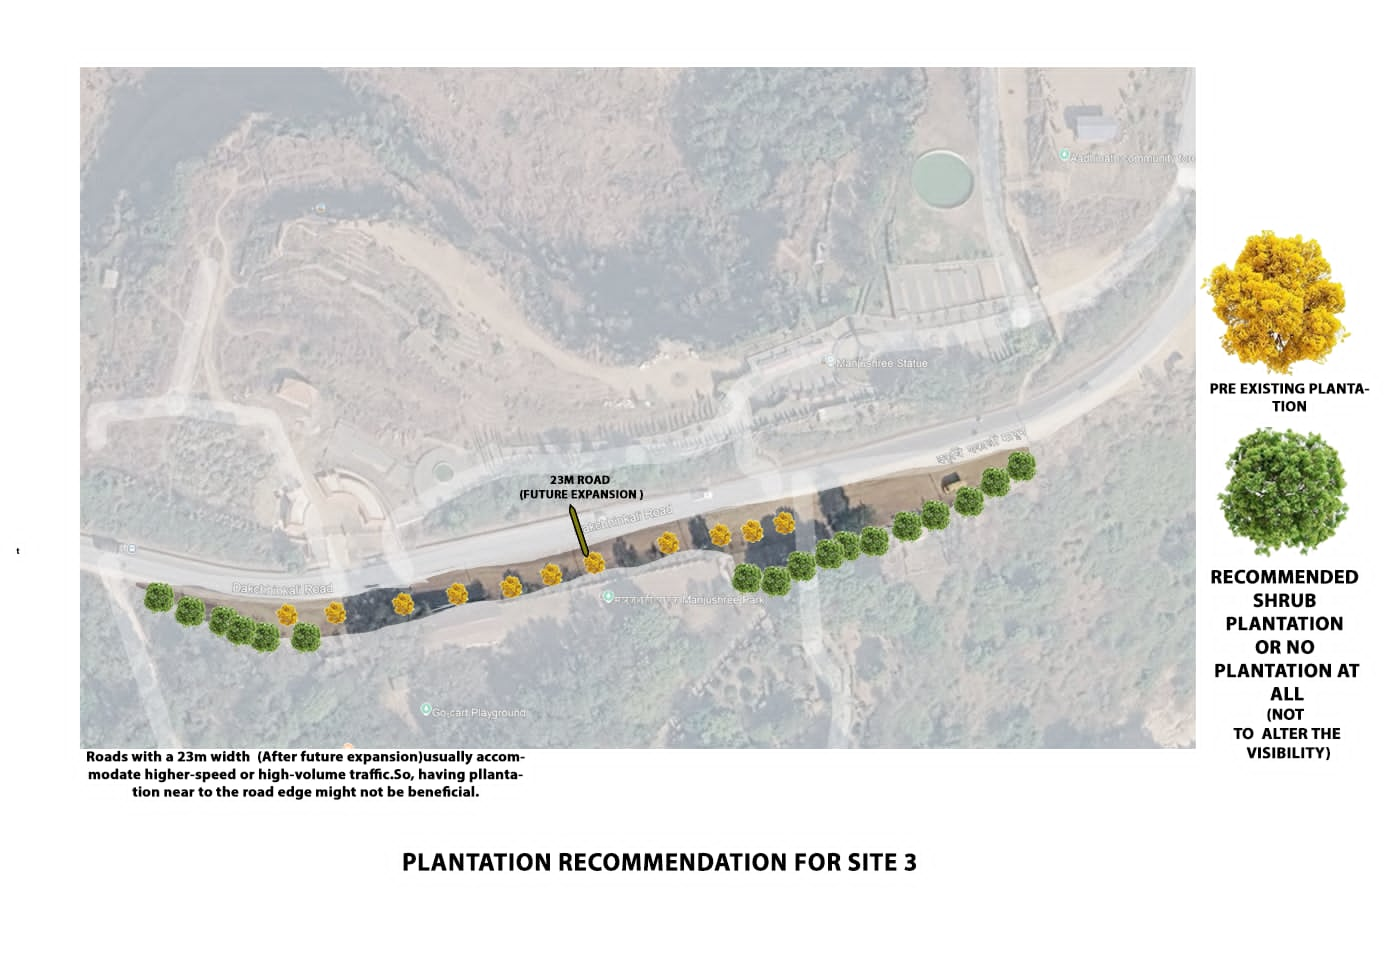
\includegraphics[width=0.78\linewidth]{site3_roadside.jpg}
  \caption{Site~3 plantation recommendation along Dakchhinkali Road. The annotated marker on the figure indicates the planned \textbf{23~m road (future expansion)} corridor, which will typically carry higher-speed and higher-volume traffic. The legend (right of figure) identifies \textbf{yellow} = \emph{pre-existing plantation} (retained roadside trees) and \textbf{green} = \emph{recommended shrub plantation, or no plantation at all}, kept low enough not to alter driver visibility. Because the right-of-way will be widened, trees planted close to the current road edge would be lost during expansion; a discontinuous low shrub line, or deferral of planting entirely, is therefore preferred over taller stock.}
  \label{fig:site3}
\end{figure}

\subsection{Recommendation}
\begin{itemize}
  \item \textbf{Preferred:} a discontinuous \textbf{low shrub} plantation that does not alter driver visibility and can be retained or relocated easily during road widening.
  \item \textbf{Alternative:} \textbf{no plantation at all} within the future right-of-way, deferring greening of this strip until after the road expansion is finalised.
  \item Pre-existing roadside trees (e.g.\ Jacaranda) remain undisturbed and are not affected by this recommendation.
\end{itemize}

% =====================================================================
\section{Engineering Considerations}
\label{sec:engineering}

\subsection{Root-System Management}
All trees planted within \textbf{3~m} of the flagstone paving or shelter foundation must have \textbf{deep tap-root} systems (e.g.\ Guava, Lapsi, Sissoo) to prevent surface heaving. Shallow-rooted species such as \emph{Eucalyptus} are explicitly excluded from this proposal.

\subsection{Utility-Line Clearance}
Utility and power lines run along the Dakchhinkali Road corridor directly adjacent to Site~3. Therefore:
\begin{itemize}
  \item No shrub or tree in Site~3 shall exceed \textbf{1.5~m} mature height, and the future 23\,m right-of-way must remain clear of any new planting.
  \item For Sites~1 and~2, trees must be planted at a minimum horizontal offset of \textbf{3~m} from any overhead line and shall not exceed 8~m mature height where lines are present.
  \item Tall species (Walnut, Alder, Sissoo), where used at all, must be set back well within the community forest, away from the road and utility corridor.
\end{itemize}

\subsection{Slope \& Drainage}
The central slope has a natural gradient of approximately 5--8\%. No grading or terracing is required. Trees planted on the downslope side should be staked securely for the first two growing seasons.

\subsection{Right-of-Way \& Road Expansion}
The planned widening of Dakchhinkali Road to \textbf{23\,m} is the principal external constraint on the design. Sites~1 and~2 sit \emph{outside} the future right-of-way and are therefore unaffected; their mature trees will not require removal. Site~3 sits \emph{within} the future right-of-way and is intentionally restricted to a low shrub line (or no planting) so that nothing of lasting value is lost when the road is widened. Any pre-existing roadside trees outside the new corridor are retained as-is.

\subsection{Comparative Engineering Specification}

\begin{table}[H]
\centering
\small
\begin{tabularx}{\linewidth}{L{3.4cm} X X X}
\toprule
\textbf{Parameter} & \textbf{Site~1 (Children's Park)} & \textbf{Site~2 (Community Forest)} & \textbf{Site~3 (Roadside)} \\
\midrule
Max tree height & 6--8~m (edges); play zone unplanted & 8--10~m (no overhead lines) & $\le$1.5~m shrub line, or none \\
Root system & Deep tap-root preferred near paths & Any; broader roots acceptable & Shallow, removable shrubs only \\
Spacing & 2--3~m (N edge); 4--5~m (S edge fruit) & 5--6~m (orchard layout) & N/A (discontinuous shrubs) \\
Planting pit size & $60 \times 60 \times 60$~cm & $60 \times 60 \times 60$~cm & $40 \times 40 \times 40$~cm \\
Soil amendment & 50\% original + 30\% compost + 20\% coarse sand & 50\% original + 40\% compost + 10\% coarse sand & Minimal \\
Staking required & Yes, bamboo, 2 seasons & Yes, bamboo, 1--2 seasons & Not required \\
Road clearance & N/A (set inside park) & N/A & Min 1.5~m from future 23~m edge \\
Utility clearance & Min 3~m horizontal & Min 3~m horizontal & Min 1.5~m horizontal \\
\bottomrule
\end{tabularx}
\caption{Engineering specification by site.}
\end{table}

% =====================================================================
\section{Technical Methodology for Fruit Plantation}
\label{sec:methodology-fruit}

Fruit trees require greater initial care, precise spacing, and nutrient-rich soil than standard forest trees in order to ensure survival and future fruiting.

\subsection{Phase 1: Site Layout \& Spacing}
A square or staggered triangular grid is recommended for the Site~2 orchard. The same spacing logic applies to the fruiting species on the southern edge of Site~1. Crowding fruit trees reduces sunlight and yields and increases pest vulnerability.
\begin{itemize}
  \item Guava, Peach, Plum, Pear: $5~\text{m} \times 5~\text{m}$ (\textasciitilde 16~ft $\times$ 16~ft).
  \item Lapsi, Lychee: at least $6~\text{m} \times 6~\text{m}$ due to large mature canopy.
\end{itemize}

\subsection{Phase 2: Pit Excavation \& Soil Conditioning}
\begin{enumerate}
  \item \textbf{Pit size:} dig larger pits than for forest stock, $0.75~\text{m} \times 0.75~\text{m} \times 0.75~\text{m}$.
  \item \textbf{Layering \& conditioning:} mix excavated topsoil with organic compost / farmyard manure (FYM) and \emph{neem cake} (\emph{Neem ko Khali}) in a 1:1 ratio. Neem cake is critical to prevent termites and root-rot diseases.
  \item Add a handful of bone meal or phosphate to encourage rapid initial root development.
\end{enumerate}

\subsection{Phase 3: Plantation Execution (Environment Day)}
\begin{enumerate}
  \item \textbf{Graft union management:} most quality fruit saplings (citrus, peach, plum) are grafted. Ensure the graft union (the bump on the lower stem) sits at least \textbf{2--3 inches above} the final soil level. Burying the graft union causes the tree to rot or lose its fruiting characteristics.
  \item \textbf{Basin preparation:} create a wide, ring-like soil depression (\emph{th\=apal\=a}) of radius $\sim$0.5~m around each tree to act as a water-harvesting basin.
  \item \textbf{Mulching:} immediately after watering, cover the basin with a 2-inch layer of dry grass or straw. Mulching retains soil moisture, suppresses weeds, and regulates soil temperature.
\end{enumerate}

\subsection{Phase 4: Long-Term Sustainability \& Protection}
\begin{itemize}
  \item \textbf{Tree guards:} sturdy, tall bamboo tree guards are mandatory. Without them, saplings will almost certainly be trampled or damaged within weeks.
  \item \textbf{Handover protocol:} as a Worldlink CSR event, a \textbf{1-year maintenance protocol} should be formalised with the Manjushree Park caretakers and CFUG. Fruit trees require regular watering through the first winter dry season to survive until the next monsoon.
\end{itemize}

% =====================================================================
\section{Park Design Recommendations (Supporting Notes)}
\label{sec:park-design}

The following items complement the Site~1 Children's Park design (Section~\ref{sec:site1}) and the Site~2 edge plantation (Section~\ref{sec:site2}). Where any item below conflicts with the Children's Park design, the Children's Park design prevails.

\subsection{Land Preparation}
Level the uneven grassy field to create a clean base for pathways, seating, and plantations; retain some natural contours where possible for character and drainage.

\subsection{Green Wall \& Boundary Treatment}
Use climbing plants (e.g.\ ivy, bougainvillea, local creepers) along walls and fences to soften hard edges and blend the park with the surrounding landscape.

\subsection{Plantation Strategy}
\begin{itemize}
  \item Avoid very large canopy trees that could block views or reduce usable space.
  \item Opt for medium-sized ornamental trees (Jacaranda, Gulmohar, Amaltas) and flowering shrubs for seasonal colour.
  \item Introduce butterfly-attracting plants (lantana, milkweed, marigold) in clusters.
  \item Where space allows, plant additional fruit-bearing trees (guava, pomegranate, citrus) for ecological and community value.
\end{itemize}

\subsection{Pathways \& Circulation}
Lay permeable stone pathways to reduce water runoff and maintain a natural look. Curved paths can guide visitors toward seating areas, gazebos, or scenic viewpoints.

\subsection{Seating \& Relaxation}
Construct shaded sitting areas (gazebos, pergolas, benches under small trees) strategically placed near plantations for a cool, relaxing environment. A central lawn can support yoga, picnics, or small gatherings.

\subsection{Wildlife-Friendly Features}
Install birdhouses on trees or poles to attract local species, and create small ecological pockets with flowering plants to encourage butterflies and pollinators.

\subsection{Water \& Sustainability}
\begin{itemize}
  \item Where feasible, add a small pond or fountain to enhance tranquillity and support aquatic plants.
  \item Integrate rainwater harvesting for irrigation.
  \item Provide composting bins to recycle organic waste into fertiliser for the plantations.
\end{itemize}

\subsection{Information \& Awareness}
Place plant information boards to educate visitors about species and their benefits. Display park rules at entry points to ensure cleanliness, safety, and respect for nature.

% =====================================================================
\section{Summary \& Approvals}
\label{sec:summary}

\begin{notebox}[CFUG Approval]
All three sites (Site~1 Children's Park, Site~2 Community Forest edge, Site~3 Roadside strip) have been confirmed by the CFUG President for the Worldlink Environment Day 2026 plantation.
\end{notebox}

\paragraph{Deliverables.} On Environment Day, the implementation team will:
\begin{enumerate}
  \item Establish Site~1 Children's Park: install log balancing trails, sand pits and timber climbing frames on curvilinear turf islands; plant the slender-tree northern boundary, the flowering / fruit southern boundary and the low spherical hedge line; lay the paved walkway and place rustic log benches.
  \item Plant Site~2 with the fruit / flowering edge species (Lapsi, Pear, Peach, Plum, Lychee, Guava) and a hedge line for demarcation.
  \item Limit Site~3 to a low shrub line (or defer planting entirely) within the future 23\,m road right-of-way.
  \item Install bamboo guards and water basins around each sapling.
  \item Hand over a 1-year maintenance protocol to the CFUG and park caretakers.
\end{enumerate}

\paragraph{Expected outcome.} A safe, attractive, low-maintenance three-site plantation centred on the Natural Playground at Site~1, supported by the Site~2 sensory edge plantation and a sightline-respecting Site~3 roadside treatment, that meets road-safety and utility-clearance constraints, supports local biodiversity, and provides an educational, edible landscape for the Chobhar community.

% =====================================================================
\section{Future Scope}
\label{sec:future-scope}

Beyond the Environment Day 2026 plantation, the Site~1 Children's Park offers significant potential for phased enhancement in subsequent CSR cycles. While the core design favours a Natural Playground (log balancing trails, sand pits and timber climbing frames), a follow-on phase may extend the play offer with conventional equipment where ground conditions and supervision permit.

\begin{itemize}
  \item \textbf{Playground equipment installation.} Subject to a fresh site-applicability check and CFUG approval, age-appropriate playground materials, such as swings, slides, see-saws, climbing frames, balance beams and an additional sandpit, may be installed within the cleared Site~1 zone. Selection and placement must respect the existing curvilinear geometry, the slender-tree northern boundary, the southern sensory plantation and the paved walkway, so that equipment is integrated \emph{around} the natural play features rather than displacing them.
  \item \textbf{Safety surfacing.} Where equipment is installed, impact-absorbing surfacing (rubber tiles, engineered wood-chip or compacted sand) should be specified beneath swings, slides and climbing structures in accordance with standard playground safety norms.
  \item \textbf{Shaded seating and gazebos.} Additional permanent benches, pergolas and a small gazebo can be added near the walkway and the southern sensory edge for caretakers and visitors.
  \item \textbf{Educational signage and a nature trail.} Species labels along the southern fruit row, a short interpretive trail and information boards on the Chobhar limestone geology and the Manjushree legend can convert the park into a low-key learning space.
  \item \textbf{Rainwater harvesting and composting.} A small harvesting tank fed from any future shelter roof, together with on-site composting bins, would close the irrigation and organic-waste loop for the Site~1 edges and the Site~2 orchard.
  \item \textbf{Lighting and security.} Solar-powered low-level path lighting along the Site~1 walkway and a basic perimeter fence around the cleared zone would extend safe usable hours and protect saplings and play equipment.
\end{itemize}

All future-scope items are conditional on a fresh site-applicability check (ground conditions, slope, accessibility and CFUG consent) at the time of implementation.

\end{document}
